\documentclass{article}

% ------------------------------------------------------------------
% ICLR 2027 submission (double-blind).
% Build: tectonic main.tex  (or pdflatex/bibtex).
% NOTE: iclr2027_conference.sty here is a PLACEHOLDER adapted from the
% bundled NeurIPS 2026 style so this draft compiles. Replace it with the
% OFFICIAL ICLR 2027 style file from OpenReview before final submission.
% ------------------------------------------------------------------
\usepackage{iclr2027_conference,times}
% \iclrfinalcopy  % uncomment for the camera-ready (non-anonymous) version

\usepackage[utf8]{inputenc}
\usepackage[T1]{fontenc}
\usepackage{hyperref}
\usepackage{url}
\usepackage{booktabs}
\usepackage{amsmath,amssymb,amsfonts}
\usepackage{microtype}
\usepackage{xcolor}
\usepackage{graphicx}
\usepackage{tikz}
\usetikzlibrary{arrows.meta,positioning,fit,backgrounds,calc}
\usepackage{pgfplots}
\pgfplotsset{compat=1.18}

% Figure accent colors (print- and CVD-safe; see docs/novelty-and-positioning.md).
\definecolor{figblue}{HTML}{2A78D6}
\definecolor{figorange}{HTML}{EB6834}
\definecolor{figink}{HTML}{0B0B0B}
\definecolor{figmuted}{HTML}{9A9A93}

\newcommand{\kc}{\textsc{kc}}
\newcommand{\regret}{\mathcal{R}}

\title{An In-Silico Instrument for Pre-Validating Corpus-Bounded Instruction:
Reference-Policy Transfer Measurement with Bidirectional Corpus-Gap and Leakage Diagnosis}

% Double-blind submission (ICLR): anonymous author block.
\author{Anonymous authors \\ Paper under double-blind review}

\begin{document}
\maketitle

\begin{abstract}
When a model answers correctly with a corpus in context, did it \emph{need} the corpus, or
did it already know the answer? We present an \emph{in-silico measurement instrument} that
answers this---and the dual question of whether a corpus is \emph{sufficient}---as a
behavioral task outcome, before any human-subject study. The central quantity is
\emph{corpus necessity}: ablate a corpus item and measure the change in a task outcome scored
against a reference. Our headline contribution is that we make necessity \emph{non-confounded}
by calibrating it against a \emph{known parametric baseline}: we \emph{construct} the ground
truth by teaching a fact into a model's weights and showing necessity falls as a
\emph{dose-response}. We demonstrate this in \textbf{two domains with independent objectives},
one of which uses \emph{no simulator at all}: (i) a control-regret simulator (maritime
collision avoidance), where teaching a hidden charted hazard into the weights collapses
necessity from a full-barrier swing to $\approx 0$, with the LoRA-scale and training-checkpoint
gradients agreeing; and (ii) a simulator-free \emph{fictional-fact question answering} task
scored by an answer checker, where teaching invented facts into a 7B model drives necessity
\emph{smoothly and monotonically from $1.00$ to $0.03$}.

This calibrated necessity measure is
the basis of two products: a \emph{corpus diagnosis} that ranks each item by necessity,
localizes which item is missing from task failures, and---crucially---splits an unrelied-upon
item into \emph{redundant} (the model already knows it) versus \emph{unusable} (the model
fails even with it present); and a \emph{corpus-sufficiency} verdict that surfaces
\emph{false sufficiency}---a corpus that only appears sufficient because the model is coasting
on priors and is therefore fragile to distribution shift.

Unlike faithfulness (RAGAS) and
context-attribution (ContextCite), which measure whether context \emph{supported} or
\emph{influenced} an output, we measure whether the model \emph{needed} it, against a
weight-level baseline they lack. The method is \emph{closed-model compatible} (API access
only) and operates \emph{per item}. As breadth we report: a \emph{learner ladder} that reads corpus
contribution beyond mere existence---decision \emph{quality} (avoiding well, not just avoiding) and
\emph{reasoning depth} (using a local rule that overrides a reflex, not just looking one up);
cross-model discrimination across current LLMs; a second control domain (roadside tire change);
\kc$\to$single-metric identifiability and estimator-recovery calibration; and a machine-unlearning arm
that yields a \emph{says\,$\neq$\,does} dissociation (gentle unlearning changes what a model \emph{says}
but not what the instrument sees it \emph{do}) as supporting weight-level evidence. All results
are \textbf{simulation-based mechanism evidence, not human-subject external validity}; we
scope the contribution accordingly and pre-register the human study as future work.
\end{abstract}

\section{Introduction}
Generic retrieval-augmented (RAG) assistants optimize for semantic relevance: give a
plausible answer to whatever is asked. That objective is wrong for training in
safety-critical procedural domains, where a semantically accurate answer can still be
instructionally wrong---delivered at the wrong complexity, skipping a prerequisite, or
worse, confidently fabricated. A growing body of work therefore builds
\emph{corpus-bounded} tutors that abstain outside a curated corpus. But a designer who has
built such a system faces a prior question: \emph{does the mechanism work?} Does the tutor
actually rely on its corpus, and does the corpus actually cover the domain? Answering this
by human-subject study is slow and expensive, and a null result there conflates many
causes.

We argue that the \emph{mechanism} of a corpus-bounded method can be falsified cheaply and
in silico, and we build the instrument to do it (Figure~\ref{fig:instrument}). Our contribution is a
\emph{methods/measurement} one, not a new tutor and not a new collision-avoidance
technique. Concretely:

\emph{The central storyline} (Sections~\ref{sec:diagnosis}--\ref{sec:weightlevel}):

\begin{itemize}
  \item \textbf{Necessity, calibrated by construction.} We measure \emph{corpus necessity}---the
  change in a task outcome when a corpus item is ablated---and make it non-confounded by
  \emph{constructing} the parametric baseline: teach a fact into the weights and necessity falls
  as a \emph{dose-response}. We show this in \textbf{two domains with independent objectives},
  one \emph{simulator-free}: a control-regret simulator (teaching a hidden hazard collapses
  necessity to $\approx 0$; LoRA-scale and checkpoint gradients agree) and a simulator-free
  fictional-fact QA task scored by an answer checker (teaching invented facts drives necessity
  smoothly $1.00\!\to\!0.03$ on a 7B model). This is a known-groups validation of the measure.
  \item \textbf{The corpus diagnosis} ranks each item by necessity, localizes a missing item from
  task failures, and splits an unrelied-upon item into \emph{redundant} (already known) versus
  \emph{unusable} (present but the model fails with it)---distinct fixes (prune vs.\ fix the model).
  \item \textbf{Corpus sufficiency}, the product face of the audit, surfaces \emph{false
  sufficiency}: a corpus that only looks sufficient because the model coasts on priors (necessity
  $\approx 0$ everywhere), a fragility ordinary RAG metrics report as all-green.
\end{itemize}

\emph{Additional breadth} (supporting the above, not the headline): a \emph{transfer instrument}
that scores a learner by its \emph{regret against a reference-policy solver} with
\kc$\to$single-metric identifiability (Section~\ref{sec:instrument}); a \emph{learner ladder} that
shows the same instrument reads corpus contribution beyond existence---decision \emph{quality} and
\emph{reasoning depth} (Section~\ref{sec:depth}); a second control domain and
estimator-recovery calibration; cross-model discrimination on current LLMs
(Section~\ref{sec:diagnosis}); and a machine-unlearning arm that yields a \emph{says\,$\neq$\,does}
dissociation as secondary weight-level evidence (Appendix~\ref{app:unlearning}).

Our contribution is a \emph{methods/measurement} one, not a new tutor. Every \emph{component} we
build on is prior art; the \emph{calibrated necessity measure} and its \emph{corpus-value/sufficiency
audit} are the open ground (Section~\ref{sec:related}). We are explicit throughout that our
evidence is simulation-based: it tests whether the machinery behaves as designed, not whether
humans learn more.

\paragraph{Organization: four case studies.} The empirical work is a register of experiments grouped
into four case studies (Table~\ref{tab:casemap}), which we reference throughout as CS$X.Y$.
\textbf{CS1} builds and stress-tests the necessity instrument on the COLREG core (the corpus
diagnosis and sufficiency products, Section~\ref{sec:diagnosis}). \textbf{CS2} climbs a
\emph{learner ladder}---blind, naive, implementer, reasoner---to show the same instrument reads not
just \emph{existence} (did you avoid at all) but \emph{quality} (did you avoid well) and
\emph{reasoning depth} (do you generalize a local rule), Section~\ref{sec:depth}. \textbf{CS3}
enriches for reach and generality (a simulator-free second domain, a discrete procedural domain, real
charted hazards). \textbf{CS4} validates the instrument itself (construct validity, reweighting
sensitivity, the unlearning null, an offline reproduce runner). The headline necessity claim is
validated by construction in two domains with independent objectives: CS1.7 (control-regret, the
large-effect known-groups endpoints) and CS3.2 (simulator-free fact-QA, the graded monotone curve).

\begin{table}[t]
\centering\small
\begin{tabular}{@{}llp{0.44\linewidth}@{}}
\toprule
Case study & Where & Key experiments (CS$X.Y$) \\
\midrule
\textbf{CS1} necessity instrument (COLREG core) & \S\ref{sec:diagnosis} &
1.1 reference-learner recovery; 1.2/1.3 cross-model leakage \& hazard discrimination;
1.4 geometric hazard suite (necessity as a fraction); 1.5 redundant-vs-unusable;
1.6 corpus-value audit/localization; 1.7 hazard dose-response
(\S\ref{sec:construction}); 1.8 sufficiency \& false-sufficiency \\
\addlinespace
\textbf{CS2} blind$\to$expert ladder (quality$\to$reasoning) & \S\ref{sec:depth} &
2.1 decision-quality band (the middle band); 2.2 reason-vs-implement (generalization axis) \\
\addlinespace
\textbf{CS3} enrichments (reach \& generality) & \S\ref{sec:diagnosis},\,\ref{sec:construction} &
3.1 real-hazard screen; 3.2 fact-QA necessity (no simulator); 3.3 discrete procedural domain
(\S\ref{sec:instrument}); 3.4 probe-suite breadth \\
\addlinespace
\textbf{CS4} validations (does the instrument hold up?) & \S\ref{sec:instrument},\,App.~\ref{app:unlearning} &
4.1 construct validity; 4.2 reweighting sensitivity ($\tau{=}1.00$); 4.3 unlearning null
(says\,$\neq$\,does); 4.4 offline reproduce runner \\
\bottomrule
\end{tabular}
\caption{The experiment register, grouped into four case studies and referenced as CS$X.Y$
throughout. The sections cut across the case studies (the instrument's forward validation, CS4/CS3.3,
is Section~\ref{sec:instrument}; its backward necessity use, CS1, is Section~\ref{sec:diagnosis}; the
weight-level calibration, CS1.7/CS3.2, is Section~\ref{sec:weightlevel}, with the CS4.3 unlearning null in
Appendix~\ref{app:unlearning}); this map is the reading guide.}
\label{tab:casemap}
\end{table}

\begin{figure}[t]
\centering
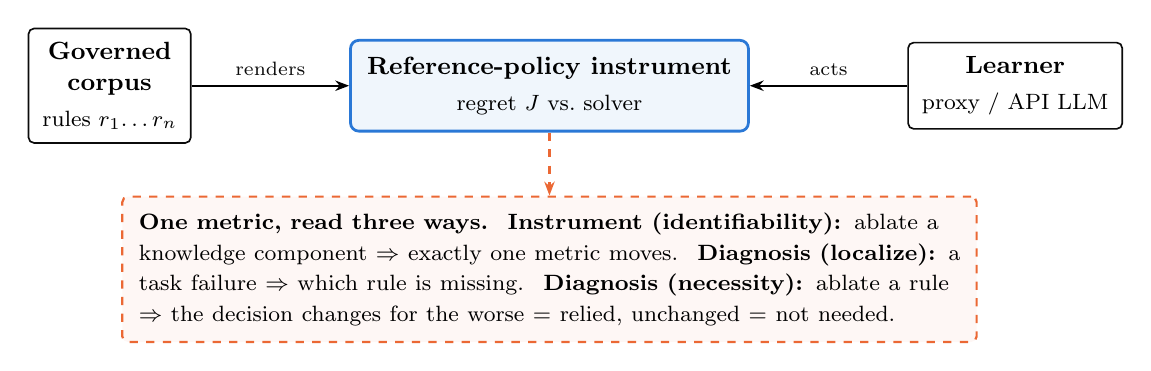
\begin{tikzpicture}[font=\small,
  box/.style={rounded corners=2pt, draw=figink, line width=0.6pt, align=center, inner sep=5pt},
  instr/.style={rounded corners=3pt, draw=figblue, line width=1pt, align=center, inner sep=6pt, fill=figblue!7},
  flow/.style={-{Stealth[length=5pt]}, line width=0.8pt},
  lbl/.style={font=\scriptsize, text=figink, align=center}]
\node[box] (corpus) {\textbf{Governed}\\\textbf{corpus}\\[2pt]{\footnotesize rules $r_1\!\dots r_n$}};
\node[instr, right=20mm of corpus] (sim) {\textbf{Reference-policy instrument}\\[2pt]{\footnotesize regret $J$ vs.\ solver}};
\node[box, right=20mm of sim] (learner) {\textbf{Learner}\\[2pt]{\footnotesize proxy / API LLM}};
\draw[flow] (corpus) -- node[lbl,above]{renders} (sim);
\draw[flow] (learner) -- node[lbl,above]{acts} (sim);
\node[draw=figorange, rounded corners=2pt, line width=0.8pt, dashed, fill=figorange!5,
      align=left, below=8mm of sim, inner sep=6pt, text width=0.86\linewidth] (diag)
  {\footnotesize\textbf{One metric, read three ways.}\;
   \textbf{Instrument (identifiability):} ablate a knowledge component $\Rightarrow$ exactly one metric moves.\;
   \textbf{Diagnosis (localize):} a task failure $\Rightarrow$ which rule is missing.\;
   \textbf{Diagnosis (necessity):} ablate a rule $\Rightarrow$ the decision changes for the worse $=$ relied, unchanged $=$ not needed.};
\draw[flow, figorange, dashed] (sim) -- (diag);
\end{tikzpicture}
\caption{The instrument, used bidirectionally. A governed corpus and a learner both feed one
reference-policy simulator that scores the learner's \emph{regret} $J$ against an automatic
solver. The same metric is then read three ways---to verify \kc$\to$single-metric
identifiability (the \emph{instrument}), to localize a missing rule from task failures, and to
detect parametric leakage by rule ablation (the \emph{diagnosis})---needing only API access to
the learner. The diagnosis is the instrument run backwards, not a separate tool.}
\label{fig:instrument}
\end{figure}

\section{Related work and positioning}
\label{sec:related}
Each strand below is established prior art; we reuse it as infrastructure and mark where our delta departs from it.

\paragraph{Learner modeling and instructional theory.} Knowledge tracing
\citep{corbett1994bkt}, the Elo rating system for adaptive systems \citep{pelanek2016}, the
Knowledge-Learning-Instruction framework \citep{koedinger2012kli}, open learner models
\citep{bull2007olm}, and the Zone of Proximal Development \citep{vygotsky1978} are all
established. We reuse them as infrastructure, not as contributions.

\paragraph{Corpus-bounded tutoring, leakage, and faithfulness.} RAG tutors that abstain
outside a corpus are standard engineering. A large line asks whether a model uses provided
context or parametric memory: faithfulness metrics score whether an answer is grounded in
context \citep{ragas2023}; context attribution ablates context sources and measures the
change in output probability to attribute a generation to them \citep{contextcite2024,
priordominance2026}; knowledge-conflict work studies which side wins when context contradicts
memory \citep{knowledgeconflicts2024, faithfulrag2025}; leakage-free benchmarking filters
items answerable with no context \citep{seedrg2026}; and intermediate-step scoring looks
beyond the final answer \citep{cuer2026}. All of these measure whether context
\emph{influenced} the output, judged on \emph{answer text}, per answer or system-wide. We
differ on three axes: (a) we score a \emph{behavioral task outcome} against a reference-optimal
policy, not answer text; (b) we attribute \emph{per corpus rule} and localize which rule is
missing or wrong, not per token or system-wide; and (c) we measure not merely \emph{influence}
but \emph{necessity}---calibrated by manipulating the parametric baseline directly (weight-level
construction and unlearning, Section~\ref{sec:weightlevel}), so a fact the model already knew is
not mistaken for one it relied on. The gap is structural: a faithfulness score is a function of the
\emph{(question, context, answer)} triple computed with the corpus \emph{present}, whereas necessity is
a \emph{contrast}---$\mathrm{acc}(\text{with corpus})-\mathrm{acc}(\text{without corpus})$---and RAGAS
never runs the without-corpus arm, so it is \emph{structurally blind} to the quantity: a model that
knows a fact and one that does not both score high with the corpus present, and the redundant case is
reported as sufficient---the false-sufficiency failure our measure is built to catch. (Our released
harness computes both side by side.) \textbf{ContextCite} \citep{contextcite2024} is the closest relative: because
it ablates context and measures the change in the response's log-probability against the model's own
baseline, it \emph{partially} tracks necessity---but it requires open weights and per-token
log-probabilities (so it cannot run on the closed API models our necessity test does), attributes
text-influence rather than a task outcome, carries no weight-level known-groups calibration, and
yields no \emph{redundant}/\emph{unusable} split or sufficiency verdict. That join is the
\emph{Corpus Diagnosis}.

\paragraph{Objective competency instruments.} Deviation-from-optimal scoring appears in
flight \citep{zinn2023flight} and construct-validity-by-novice/expert-separation in surgery
\citep{vandongen2007lapsim}; control-theoretic notation has been applied to knowledge
dynamics \citep{controlkt2024}; regret is used in RL transfer \citep{transferregret2024};
maritime training analytics regress simulator measures onto instructor ratings
\citep{maritime2025}. None uses a \emph{reference solver's regret} as the
\emph{learner} transfer outcome with \kc$\to$single-metric identifiability. That is the
\emph{Transfer Instrument}.
We borrow mature maritime-autonomy tooling---velocity obstacles \citep{fiorini1998vo} and
simulation-based MPC \citep{johansen2016sbmpc}---purely as reference solvers, never as a new
collision-avoidance method \citep{colregcompliance2024,imo1972colregs}.

\paragraph{Proxy learners.} Simulated students have long authored and evaluated tutors; LLM
student agents now pilot assessment items \citep{luwang2024} and simulate learners for
tutoring-system development \citep{agent4edu2025}, and controlled variants suppress knowledge
by prompting \citep{apartsin2026}, interpolate parametric competence \citep{ps2_2026}, or
unlearn a model into a novice \citep{song2026unlearn}. Pre-deployment simulated-learner
screens have very recently appeared \citep{llmjudgeaudit2026,educlaw2026}. We therefore
\emph{demote} the proxy-learner idea to an application: our narrow residual claim is running
\emph{two complementary proxy classes} (parametric competence \emph{and} unlearned LLM)
scored on the \emph{same regret-to-reference instrument} the human trial would use---which
none of these do.

\section{The Transfer Instrument}
\label{sec:instrument}
This section defines and verifies the instrument's \emph{forward} use---measuring transfer and skill.
The \emph{backward} use that measures corpus necessity, the paper's central contribution, follows in
Section~\ref{sec:diagnosis}; the construct-validity, identifiability, and robustness checks below are
the support that licenses it.

\paragraph{Task and metric.} The worked domain is COLREG collision avoidance: a
power-driven vessel must choose course and speed to resolve an encounter. We implement a
kinematic simulator with an elliptical ship domain and a Collision Risk Index, and two
reference solvers---velocity obstacles \citep{fiorini1998vo} and simulation-based
MPC \citep{johansen2016sbmpc}. For a learner policy $\pi$ on scenario set $S$ we define the
transfer outcome as regret against a reference policy $\pi^\star$,
\begin{equation}
  \regret(\pi) \;=\; \frac{1}{|S|}\sum_{s \in S}\big[\, J(\pi, s) - J(\pi^\star, s)\,\big],
\end{equation}
where $J$ is the per-encounter objective (a weighted sum of a safety-margin barrier, COLREG
compliance penalty, and route deviation; lower is better) and $\pi^\star$ is the reference
maneuver. Unlike item correctness, $\regret$ is continuous, objective, and instructor-free.

\paragraph{On ``reference,'' not ``optimal.''} We deliberately avoid claiming a global
optimum. VO and SB-MPC are strong, widely-used near-optimal solvers, but neither is proven
globally optimal for the full nonconvex encounter; calling their output ``optimal'' would
overclaim. The instrument does not need a true optimum---only a reference that construct
validity shows separates naive from expert behavior (below). Regret is thus measured
against a fixed, reproducible reference policy, and we report which solver is used.

\paragraph{Construct validity and metric grading.} The instrument must separate good from
bad policies before any learning claim, and---if it is to be a transfer measure rather than
a pass/fail check---the metric must \emph{grade}, not collapse to two values. Across a
varied set of nine encounters (head-on, starboard/port crossing, overtaking, and
restricted-visibility geometries), three policies of increasing competence separate cleanly
and continuously on $J$ (Table~\ref{tab:construct}): a naive hold-course policy
(mean $J\approx1765$, clearing only $11\%$ of domains), a velocity-obstacle reference
($J\approx0.70$, all clear), and SB-MPC ($J\approx0.01$). The objective takes $20$ distinct
values in $[0.00, 1995.18]$ over the policy$\times$scenario cells---a graded metric, with
the safe regime (VO/SB-MPC) itself spanning a continuous $0.00$--$1.27$ range. On the
discrete procedural domain the same logic holds: an expert policy scores $J=0$ against a
reckless $J=200$ with the safety violation caught. This is the novice/expert-separation
logic of \citet{vandongen2007lapsim}, applied to a decision/control task rather than manual
skill.

\begin{table}[t]
\centering
\small
\begin{tabular}{@{}lrrrrr@{}}
\toprule
Policy & mean $J$ & median & min & max & cleared \\
\midrule
naive (hold course) & $1765.44$ & $1988.08$ & $1.08$ & $1995.18$ & $11\%$ \\
VO reference & $0.70$ & $0.58$ & $0.33$ & $1.27$ & $100\%$ \\
SB-MPC reference & $0.01$ & $0.01$ & $0.00$ & $0.03$ & $100\%$ \\
\bottomrule
\end{tabular}
\caption{Construct validity and grading across nine varied encounters. The objective $J$
separates the three competence levels cleanly and takes a continuous range of values
(20 distinct across all cells, $[0.00, 1995.18]$)---it is a graded transfer metric, not a
near-binary check. \texttt{npm run colreg:construct}.}
\label{tab:construct}
\end{table}

\paragraph{\kc$\to$single-metric identifiability.} We design each knowledge component to
govern exactly one metric, so ablating a \kc\ degrades that metric and no other. On the
procedural domain this is \emph{exact}: each ablated competence degrades only its governed
metric, and a monotone competence$\to$performance gradient ($J:204\to 0$) follows as
competence is acquired in curriculum order; on the COLREG instrument the same gradient spans
nearly five orders of magnitude, collapsing only as the two domain-clearing competencies come
online---mean $J$ by curriculum stage ($\varnothing$, {+}give-way, {+}turn-starboard, {+}bold-turn,
\textbf{{+}act-early}, \textbf{{+}safe-speed}, {+}multi-ship) is
$1765\!\to\!1759\!\to\!1745\!\to\!1605\!\to\!\mathbf{221}\!\to\!\mathbf{0.03}\!\to\!0.03$
(\texttt{npm run colreg:construct}). Because the property holds on both a
continuous-control and a discrete-procedural instrument, it is a general measurement-design
property, not a COLREG artifact.

\paragraph{Is identifiability tautological?} A fair objection is that the mapping is a design choice, so
``ablate the \kc, that metric moves'' is true by construction. But the \emph{cross-effect} claim can
fail: designing the metrics does not guarantee that ablating one \kc\ leaves the \emph{others} unchanged
---if the objective's terms are entangled, ablation bleeds across metrics. Identifiability is the
empirically-checked \emph{absence} of that bleed, and it is what makes the Corpus Diagnosis
(Section~\ref{sec:diagnosis}) actionable (a task failure attributes to a specific rule). We thus treat it
as a design requirement to be verified per instrument. On the procedural domain the verification is clean
(Table~\ref{tab:ident}): each ablation degrades only its governed metric, maximum off-diagonal change
$0.0000$---no cross-bleed.

\begin{table}[t]
\centering
\small
\begin{tabular}{@{}lcccc@{}}
\toprule
ablated \kc\ $\downarrow$ / metric $\rightarrow$ & safety & core & sequencing & finishing \\
\midrule
safety      & $\mathbf{-1.00}$ & $0.00$ & $0.00$ & $0.00$ \\
core steps  & $0.00$ & $\mathbf{-1.00}$ & $0.00$ & $0.00$ \\
sequencing  & $0.00$ & $0.00$ & $\mathbf{-0.22}$ & $0.00$ \\
finishing   & $0.00$ & $0.00$ & $0.00$ & $\mathbf{-1.00}$ \\
\bottomrule
\end{tabular}
\caption{\kc$\to$single-metric identifiability (procedural domain). Change in each metric
after ablating each knowledge component. The diagonal (bold) is the intended governed
metric; every off-diagonal cell is $0.00$ (max $|\Delta|=0.0000$)---ablation does not bleed
across metrics. \texttt{npm run proc:identifiability}.}
\label{tab:ident}
\end{table}

\paragraph{Robustness to weighting choices.} The objective embeds weighting choices---the
elliptical ship-domain radii and the margin/compliance/deviation weights---and a fair worry
is that the competence ranking is an artifact of those choices. We falsify this with a
sensitivity analysis (\texttt{npm run colreg:sensitivity}) that holds every policy's
\emph{behavior} fixed and re-scores under $232$ perturbations: a one-at-a-time
$\pm25$--$50\%$ sweep of each parameter plus $200$ joint samples with every parameter
independently scaled in $[0.6, 1.4]$. Across the whole ensemble, both orderings are
preserved exactly---the naive policy stays worst and the six-component competence gradient
stays monotone in $J$ (Kendall $\tau=1.00$ on every perturbation, invariant rate $100\%$).
The CRI parameters are excluded because CRI is a reported diagnostic, not a term in the
scored objective, so the ranking is invariant to them by construction. The protocol's
conclusions are thus a property of the competence structure, not of the weight calibration.

Estimator-recovery and calibration on synthetic data---validating the measurement, not just the
metric---appear in Appendix~\ref{app:recovery}.

\section{The Corpus Diagnosis: the same instrument, read backwards}
\label{sec:diagnosis}
The Corpus Diagnosis is not a second tool. It is the Transfer Instrument of
Section~\ref{sec:instrument} run in reverse: the \emph{same} objective metric answers two
opposite questions. This backward reading---\emph{does the learner rely on a given corpus item?}---is
the paper's central contribution; the forward construct validity of Section~\ref{sec:instrument} is
what licenses it.

\paragraph{(i) Corpus-gap localization.} When the corpus is missing or wrong on a rule, the
learner's failures on the governed metric have a signature that attributes the failure to a
\emph{specific} rule/node. We compute, per rule, an ablation-delta---the rise in the
governed penalty when that rule is removed---and a localization that names the governed
component. A large delta plus a matching localization means the learner \emph{relied on}
that corpus rule.

\paragraph{(ii) Necessity as \emph{different and better}.} The mirror image asks whether the learner
\emph{needed} an item---read as a positive signal, not a null. Ablate the item and compare the run against
the with-corpus run on two observables (Figure~\ref{fig:diffbetter}): does the \emph{decision} change
(\textbf{different}), and does the learner \emph{succeed with} the item present (\textbf{usable})? An item
is \textbf{relied on} when the corpus changes the decision \emph{for the better}---removing it flips a
succeeding call into a failing one; if the decision is unchanged, the learner would have acted the same way
without the corpus and did not need it. Reading necessity as ``the corpus changed the call, and it helped''
is stronger than the subtractive ``nothing broke when we removed it,'' and it is read off the graded regret
instrument itself---not a decoupled side-metric---calibrated against a known parametric baseline by
construction (Section~\ref{sec:construction}), and visible per model as the reliance spectrum of
Table~\ref{tab:disc}. (A coarser categorical verdict---a majority vote that adds a counterfactual and a
closed-book baseline---is deferred to Appendix~\ref{app:verdict}.)

\paragraph{(iii) When the decision doesn't change, or changes but fails.} The three non-relied cells of
Figure~\ref{fig:diffbetter} demand different fixes: an \emph{unchanged} decision that succeeds is
\textbf{redundant} (prune it) and one that fails is \emph{ignored} (present but unused); a decision that
\emph{changes but still fails} is \textbf{unusable} (the model can't execute the rule) or flags a
\emph{misleading} item---a corpus-quality fault the subtractive ``did removing it hurt'' test cannot even
see. On the sweep (Table~\ref{tab:disc}) Opus's call changes on every hazard when the rule is removed, while
Llama-4-Maverick applies the same reflex either way and grounds on the override reaches ($4/8$ \emph{ignored},
scored \textbf{unusable}).

\begin{figure}[t]
\centering
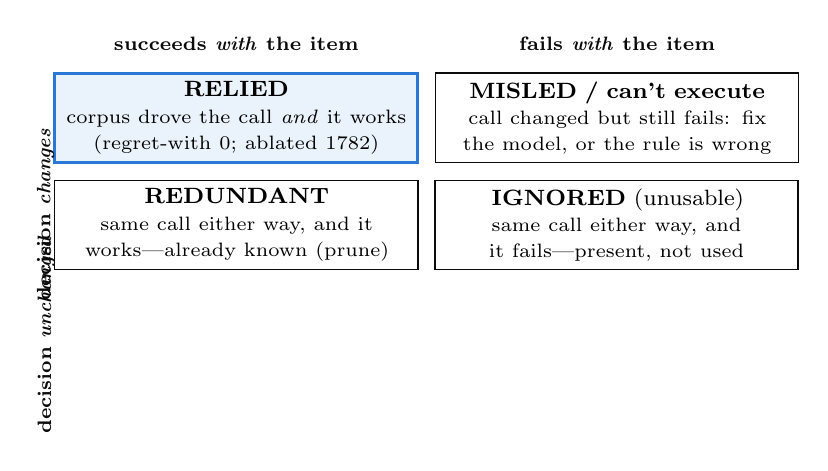
\begin{tikzpicture}[font=\footnotesize,
  cell/.style={draw=figink, line width=0.5pt, text width=44mm, align=center, inner sep=3pt, minimum height=11mm},
  relied/.style={cell, fill=figblue!10, draw=figblue, line width=1pt},
  lbl/.style={font=\scriptsize\bfseries, text=figink}]
\node[relied]                (tl) at (0,0) {\textbf{RELIED}\\{\scriptsize corpus drove the call \emph{and} it works}\\{\scriptsize (regret-with $0$; ablated $1782$)}};
\node[cell, right=2mm of tl] (tr)          {\textbf{MISLED / can't execute}\\{\scriptsize call changed but still fails: fix the model, or the rule is wrong}};
\node[cell, below=2mm of tl] (bl)          {\textbf{REDUNDANT}\\{\scriptsize same call either way, and it works---already known (prune)}};
\node[cell, right=2mm of bl] (br)          {\textbf{IGNORED} (unusable)\\{\scriptsize same call either way, and it fails---present, not used}};
\node[lbl, above=1.5mm of tl.north] {succeeds \emph{with} the item};
\node[lbl, above=1.5mm of tr.north] {fails \emph{with} the item};
\node[lbl, rotate=90, anchor=south, left=1mm of tl.west] {decision \emph{changes}};
\node[lbl, rotate=90, anchor=south, left=1mm of bl.west] {decision \emph{unchanged}};
\end{tikzpicture}
\caption{Necessity read as \emph{different}$\times$\emph{usable}: ablate an item and ask whether the
\emph{decision} changes (rows) and whether the learner \emph{succeeds with} it (columns). Only the top-left
cell is \textbf{relied on}---the corpus changed the call, for the better. Two observables replace the
necessity/regret-with/verdict stack; the categorical verdict is deferred to Appendix~\ref{app:verdict}.}
\label{fig:diffbetter}
\end{figure}

\paragraph{Corpus sufficiency, and \emph{false sufficiency}.} Rolling the per-item classifications to the
corpus level yields a sufficiency judgement for a query set: \emph{contributing} (every item
relied upon), \emph{partial}, \emph{unusable}, or---the diagnostic ordinary RAG metrics cannot
produce---\emph{false sufficiency}: task accuracy is high yet necessity is $\approx 0$ everywhere,
so the corpus is not carrying the load and success rides on priors, fragile to distribution shift.
The claim is explicitly scoped to the probed query set (sufficiency is always ``for these
queries''); the false-sufficiency signal (necessity $\approx 0$) is precisely the measurable
warning that a bounded-query sufficiency claim will not survive a shift.

\paragraph{Offline recovery of known ground truth.} Before the real-model sweep, we confirm the
classification recovers truth we control. Against two reference mock learners the instrument is exact: the
corpus-bound mock's decision \emph{changes} when the rule is ablated and it then grounds (regret $0.2$ with
the rule $\to 1981$ without $\Rightarrow$ \emph{relied}); the leaking mock's decision is \emph{unchanged}
and already clears both ways ($\Rightarrow$ \emph{redundant}).

\paragraph{Real-model discrimination (CS1.3).} We run the necessity test as a \emph{suite}: eight
independent, alternating-bow charted hazards, each isolated in its own corpus, so per-model necessity is
the \emph{fraction of the suite relied upon} (resolution $1/8$)---the fraction-valued reading of CS1.4
that supersedes an earlier single-hazard $\delta_{\regret}$ scan (kept in the released provenance).
Five production models run over AWS
Bedrock---Claude Opus/Haiku/Sonnet~4.5, Amazon Nova-micro, and Llama-4-Maverick-17B---at a temp-$0$ point
estimate plus a $K{=}5$ temp-$0.7$ ensemble (Table~\ref{tab:disc}). Three findings.

\emph{(1) A graded reliance spectrum, co-determined by ablated-arm fallback.} Necessity depends on what a
learner \emph{does when the rule is removed}. The suite is $4$ \emph{override} reaches (the hazard sits
where the default Rule-14 starboard turn grounds) $+$ $4$ where starboard already clears, so a model that
falls back on the starboard reflex when the rule is ablated is \emph{rescued} on the four non-override
reaches and caps at $4/8$ \emph{by construction}: Haiku ($4$), then Sonnet ($3$) and Nova-micro (temp-$0$
$2$, but $\approx\!0$ in the ensemble, below) reading fewer override reaches, down to Llama-4-Maverick
($0$, which grounds even with the rule present). Claude Opus is the separate case: it \emph{holds course}
when ablated rather than falling back (finding~3's strict-mode behavior), so it grounds on all $8$. The
spectrum is real cross-model range standard COLREG cannot show, but it grades reading \emph{and}
ablated-arm conservatism together---Opus's $8/8$ means it does not fall back, not that it out-reads Haiku.

\emph{(2) The decision-change reading, not the verdict.} Classifying on Figure~\ref{fig:diffbetter}'s two
observables rather than the majority-vote verdict matters: the verdict \emph{undercounts} a model whose
decision plainly depends on the fact but which answers closed-book from priors---it put Haiku at $0/8$ where
the decision-change reading gives $4/8$ (Appendix~\ref{app:verdict}).

\emph{(3) Strict-mode faithfulness on standard COLREG.} On \emph{standard} COLREG Opus's decision also
changes when the rule is ablated, but the audit log shows why, and it is not a Rule-14 knowledge gap: when
the steering rule is removed Opus \emph{abstains/holds course} (``no rules were provided\ldots'', obeying the
instruction to use only the provided rules) rather than falling back on its obvious parametric Rule-14. Haiku
instead applies the Rule-14 starboard reflex, and Sonnet varies across samples. The categorical verdict for
this case (and the strict-mode reading) is Appendix~\ref{app:verdict}; provenance
\texttt{experiments/provenance/cross-model/}.

\begin{table}[t]
\centering
\small
\begin{tabular}{@{}lccc@{}}
\toprule
Model & relied & unusable & redundant \\
\midrule
Claude Opus 4.5      & $\mathbf{8}$   & $0$            & $0$ \\
Claude Haiku 4.5     & $4$            & $0$            & $4$ \\
Claude Sonnet 4.5    & $3$            & $2^{\dagger}$  & $3$ \\
Amazon Nova-micro    & $2^{\dagger}$  & $2^{\dagger}$  & $4$ \\
Llama-4-Maverick-17B & $0$            & $4$            & $4$ \\
\bottomrule
\end{tabular}
\caption{Cross-model necessity over the eight-hazard corpus-only suite (five models, AWS Bedrock; CS1.3).
Each hazard is isolated in its own corpus, so the three counts partition the suite of $8$ and per-model
reliance is a fraction (CS1.4's fraction-valued fix, superseding an earlier single-hazard
$\delta_{\regret}$ scan). Classification uses \emph{necessity} $=\regret(\text{ablated})-\regret(\text{with-corpus})$
and \emph{regret-with}: \textbf{relied} $=$ necessity $>100$ \emph{and} regret-with $<10$ (clears with the
item, grounds without); \textbf{unusable} $=$ regret-with $\ge 10$ (grounds \emph{with} the item
present---present-but-unexploited); \textbf{redundant} $=$ otherwise (clears both ways). The thresholds
sit in wide empty gaps: the necessity signal is the clear$\leftrightarrow$ground swing
($\sim\!1400$--$1782$) against $\approx\!0$ noise, and regret-with $\ge\!10$ is a clean fail-with-corpus
cut. Values are the temp-$0$ point estimate; the $K{=}5$ temp-$0.7$ ensemble has sd $\approx\!0$ except
($\dagger$): Sonnet unusable $1.2\pm0.7$, Nova-micro relied $0.2\pm0.4$ and unusable $2.2\pm0.7$.
Counts reflect ablated-arm fallback as well as reading: reflex-appliers cap at $4/8$ (the four override
reaches), and Opus's $8/8$ reflects that it holds course rather than falling back on Rule-14 when the rule
is ablated (cf.\ finding~3). Provenance \texttt{experiments/provenance/cross-model/}.}
\label{tab:disc}
\end{table}

\paragraph{Per-rule, not just per-corpus.} To show the diagnosis attributes reliance to a
\emph{specific} rule rather than to corpus presence in general, we add a second, independent
rule---Rule~15 crossing give-way---exercised on its own crossing scenarios (a rule only
moves the metric on scenarios that invoke it, so each probe carries a matched subset).
Ablating each rule produces a large regret signal on its own encounters: on
\texttt{gemini-flash-latest} under the bound prompt, ablating Rule~14 gives
$\delta_{\!\regret}{=}1981$ (head-on) and ablating Rule~15 gives $1285$ (crossing), each localized on its
own disjoint scenario subset (\texttt{gemini-flash-lite} reproduces this at $658$/$662$), so the instrument
reads reliance per rule.

\paragraph{A real fact can be corpus-only (screen check, CS3.1).} Is ``corpus-bound'' just ``cannot know an
invented fact''? We test whether a \emph{genuine} charted danger can be corpus-only for a frontier model
with a closed-book \emph{screen}: ask Claude Opus to name each candidate unprompted and keep only those it
cannot recall. Two official-gazetteer rocks---Elwha Rock (Puget Sound) and Fullastern Rock (Antarctica)---
survive (Opus does not name them), while Whittle Rock (False Bay) is screened out (named, so parametric).
This validates the \emph{screen}---a real fact \emph{can} be corpus-only---but adds no independent necessity
\emph{magnitude}: the hazard's identity never enters $J$, so any hazard Opus reads yields the same
full-barrier $\delta_{\regret}\!\approx\!1998$ \emph{by construction}. The screen is imperfect (the Seven
Stones reef failed to screen out because Opus recalled adjacent dangers), which we report rather than force.
The load-bearing graded-and-calibrated evidence is the simulator-free fact-QA dose-response
(Section~\ref{sec:construction}, CS3.2), free of the fixed-geometry confound.

\paragraph{Presence vs.\ retrieval.} A finer decomposition---separating value the corpus \emph{holds}
from value the retriever \emph{surfaces}, over the \textsc{none}/\textsc{retrieved}/\textsc{oracle}
conditions, so a curation failure, a retrieval failure, and a priors success are distinguished---is
developed in Appendix~\ref{app:retrieval}.

\section{Case Study 2 --- from blind to expert: reading quality and reasoning depth}
\label{sec:depth}
Necessity is always measured against a \emph{learner}, so it helps to name the cast. We arrange them
on a \emph{learner ladder} of increasing corpus use---\textbf{blind} (cannot perceive the danger;
holds course and collides), \textbf{naive} (sighted but untrained; avoids, but generically---wrong
side or over-bold), \textbf{implementer} (applies a corpus rule verbatim where the situation matches
the corpus), and \textbf{reasoner} (combines the corpus with base rules and partial observation for
novel or ambiguous cases)---with an off-ladder \textbf{parametric expert} that is competent
\emph{without} the corpus (it already knows the rule in its weights; necessity $\approx 0$). Each
rung-gap is a distinct corpus contribution and a distinct measurement. Case Study~1
(Section~\ref{sec:diagnosis}) lives on the source axis---\emph{anything} vs.\ \emph{parametric
expert}, i.e.\ necessity itself. This section walks the depth ladder's lower rungs: blind$\to$naive is
the \emph{existence} gap, naive$\to$implementer the response-\emph{quality} gap (CS2.1), and
implementer$\to$reasoner the \emph{generalization} gap (CS2.2).

Perception is a second source of the information the corpus can carry, which couples \emph{what the
corpus must supply} to \emph{whether the learner can see}: an existence-corpus (``a danger is there'')
is necessary only when the learner is \emph{blind}, and a quality-corpus (``the right way to pass it'')
only when the learner is \emph{sighted} (perception already gives existence but not which-side or
how-much). This is exactly why CS1 \emph{hides} the hazard---so existence must come from the corpus and
the learner must be blind---while CS2 \emph{shows} it---so existence is free and the corpus must earn
its keep on quality.

\paragraph{CS2.1 --- decision quality (the middle band).} The transfer objective of
Section~\ref{sec:instrument} is deliberately \emph{bimodal}: a single hard barrier (collision/grounding,
$\approx 2000$) dominates the graded terms $\sim\!1000\times$, so read directly it measures
\emph{existence} (did you avoid at all), not \emph{quality} (did you avoid well). Reading quality off
its \emph{own} axis---the graded terms (ship-margin $+$ compliance $+$ route-deviation) \emph{conditional
on clearing}---separates three sailors the barrier alone conflates: \textbf{blind} collides (the barrier
fires), \textbf{naive} clears but the wrong way (quality-regret $\approx 0.87$, the middle band), and
\textbf{trained} clears lawfully (quality-regret $\approx 0.01$, the floor). A turn-angle sweep traces a
smooth graded quality surface whose minimum sits at the trained maneuver, so the middle band is a genuine
continuum, not a third discrete level. \emph{Honest note:} this graded band comes from the smooth quality
terms; a hard \emph{second} hazard (a shoal on the wrong-side escape) yields only a thin feasibility shell
rather than a graded surface, and that harder version is deferred to CS2.2's overriding cases.

\paragraph{CS2.2 --- reason vs.\ implement (the generalization axis).} The deepest rung separates two
\emph{trained} learners that are identical on textbook cases and diverge only where a corpus \emph{local
rule} must override the reflex. We add a reasoning-aware objective in which a corpus-supplied local rule
redefines the governing give-way side (COLREG Rules~2 and~9 subordinate the default steering rules to
local conditions and good seamanship); when the local rule is absent the default starboard governs, so
every prior scenario and result is unchanged. An \emph{implementer} that looks the rule up and applies it
verbatim and a \emph{reasoner} that treats the corpus as premises then behave identically where the
textbook rule already fits, and diverge only where the local rule overrides it. On a matched suite the two
are indistinguishable (implementer $\equiv$ reasoner, $\Delta$regret $0.00$); on a conflict suite built so
the safe side \emph{alternates} port/starboard---so no fixed reflex can pass---the \textbf{reasoner clears
$6/6$} while the \textbf{lookup implementer clears only the $3$} reaches where the local rule is redundant
with Rule~14 and \emph{grounds on the $3$ it overrides}. The necessity of the local-rule corpus is thus
$3/6$, separable \emph{only} on the overriding cases---the fact-vs-reasoning distinction (RAG-as-lookup
vs.\ RAG-as-reasoning-substrate) made measurable. As in CS2.1 these are hand-built reference policies
with known ground truth, so the run validates the \emph{instrument}.

\paragraph{CS2.2 (live) --- a real model reads as a reasoner.} Putting a live model through the \emph{same}
B2 rig---necessity $=\regret(\text{ablated})-\regret(\text{with-corpus})$, two conditions per reach, a
temp-$0$ point estimate plus a $K{=}5$ temp-$0.7$ ensemble---makes the model the measured \emph{subject}.
\textbf{Gemini-2.5-flash} reads as a \textbf{reasoner}. On the three \emph{override} reaches (deep water
to port, where the Rule-14 starboard reflex grounds) it relied on the local rule in $5/5$ samples,
necessity $1782\pm0$: with the corpus it alters to port and clears, and ablated it applies Rule~14 and
grounds. On the three \emph{redundant} reaches (where the local rule agrees with Rule~14) the necessity is
scattered instead (relied $1$--$2/5$, sd $\approx\!800$)---the audit log shows the model
\emph{intermittently abstains} in the ablated arm (``the situation description contains contradictory
information''\,$\to$ holds course $\to$ grounds $\to$ a spurious large necessity). \emph{Scope note:} with
only six draws per reach this is the \emph{observed} behavior, not an abstention rate; the reasoner
reading rests on the override reaches ($5/5$, zero variance), and the redundant-reach scatter is exactly
what the ensemble's variance control flags as noise rather than reliance. Provenance:
\texttt{experiments/provenance/reason-implement/gemini-2.5-flash.b2.jsonl}.

\section{Validating necessity at the weight level}
\label{sec:weightlevel}\label{sec:construction}
The necessity/leakage test infers a fact about a model's \emph{weights} from a change in the
\emph{prompt}: ablate an item from the corpus, and if the governed outcome does not move, the
model did not need it. The sharpest objection is that corpus \emph{context} removal is not
weight-level \emph{knowledge} change, so a small necessity could be the no-context heuristic in
disguise---or, conversely, a large necessity could reflect a fact the model happens not to know
for reasons we did not control. We close this primarily by \emph{construction} (below); a complementary
\emph{unlearning} cross-check---removing a rule the model \emph{does} know---is secondary, because
standard COLREG rules lack necessity range, and is deferred to Appendix~\ref{app:unlearning}.

\paragraph{Validation by construction: the necessity dose-response.}
\emph{Necessity is a non-confounded, calibrated measure}---teaching
a fact into the weights drives it down as a dose-response---so a near-zero reading is evidence the model
already knew the item, not a context-removal artifact. The decisive test is \emph{known-groups}: build
models along a gradient from fact-naive to
fact-knowing \emph{by construction}, and show necessity falls monotonically. We teach a target
fact into the weights (LoRA SFT) and sweep two independent knowledge gradients---the LoRA scale
$\alpha$ (one adapter, evaluated at $\alpha\in[0,1]$) and training checkpoints---so their
agreement rules out a gradient-method artifact. We run this in two domains with \emph{independent
objectives}, the second of which uses no simulator at all.

\paragraph{Domain 1 --- control-regret (a hidden hazard), CS1.7.} Standard COLREG rules have little dynamic
range for this test---every current frontier model already knows them (Section~\ref{sec:diagnosis})---so we
use a \emph{corpus-only charted hazard}: a danger scored by the objective barrier but not shown in
the prompt, knowable only from the corpus. Teaching it into a Qwen2.5-3B model collapses necessity
from a full-barrier swing ($\regret$-necessity $\approx 667$, naive) to $\approx 0.2$ (taught), and
the $\alpha$ and checkpoint sweeps \emph{agree} on the transition. The curve is a \emph{step}, not
graded---the correct signature for a \emph{single discrete fact}, which is learned as a threshold
(the model either lacks the fact and grounds, or has it and clears)---so the hazard arm establishes
the large-effect known-groups \emph{endpoints}, and the graded curve is Domain 2's job.

\paragraph{Domain 2 --- simulator-free fictional-fact QA, CS3.2.} We invent facts about fictional entities
(research outposts and their attributes) that no model can have memorized, and score answers with a
programmatic checker---\emph{no simulator, no reference policy}. Because the facts are fictional, a
competent model is necessarily corpus-bound at baseline, and because there are many \emph{independent}
facts, partial teaching learns a fraction of them, so the aggregate necessity is \emph{graded}.
Teaching the facts into a Qwen2.5-7B-Instruct model drives mean necessity smoothly and monotonically
down the LoRA-$\alpha$ gradient: $1.00\!\to\!0.93\!\to\!0.29\!\to\!0.03$ (Table~\ref{tab:dose}) as the
facts are internalized. A
training-checkpoint sweep reproduces the same curve ($1.00\!\to\!0.25\!\to\!0.03$)---the two gradients
are built differently (scaling one converged adapter vs.\ genuine partial training), so their
agreement rules out a gradient-method artifact. This is the clean dose-response, in a domain we did
not build a simulator for---answering the objection that the measure is an artifact of one hand-built
environment. (Necessity here is measured closed-book:
the without-corpus condition permits parametric answering, so taught knowledge surfaces rather than
being suppressed by a strict ``answer only from the provided facts'' instruction.)

\begin{table}[t]
\centering\small
\begin{tabular}{@{}lccccc@{}}
\toprule
Domain / objective & \multicolumn{5}{c}{necessity across the knowledge gradient} \\
\midrule
& naive & & & & taught \\
Hazard / $\regret$ (Qwen-3B) & $667$ & \multicolumn{3}{c}{$\cdots$ step $\cdots$} & $0.2$ \\
\midrule
& $\alpha{=}0$ & $0.25$ & $0.5$ & $0.75$ & $\alpha{=}1$ \\
Fictional-fact QA / accuracy (Qwen-7B) & $1.00$ & $0.93$ & $0.29$ & $0.03$ & $0.03$ \\
\bottomrule
\end{tabular}
\caption{Necessity dose-response by construction. Teaching a fact into the weights drives the
instrument's necessity for that fact down. The hazard (control-regret objective) gives a
large-effect \emph{step}---the known-groups endpoints for one discrete fact, with $\alpha$/checkpoint
sweeps agreeing---while the simulator-free fictional-fact QA (answer-accuracy objective) gives the
\emph{graded} monotone curve over many independent facts. Two objectives, one measure. Harness:
\texttt{experiments/unlearning} (\texttt{dose\_response.py}), \texttt{src/engine/factqa}.}
\label{tab:dose}
\end{table}

\paragraph{Two supporting arms (appendices).} Two secondary arms build on this calibrated measure. A
complementary \emph{unlearning} cross-check yields a \emph{says\,$\neq$\,does} dissociation---gentle,
guardrailed SimNPO on a 3B model suppresses what the model \emph{says} (forget-set likelihood collapses,
the Rule-14 citation disappears) while the steering \emph{decision} the instrument scores is untouched,
and an aggressive recipe instead \emph{inverts} the rule to port---a caution that weight-level unlearning
of a safety rule can produce confident non-compliance (Appendix~\ref{app:unlearning}). And the intended
use, a \emph{pre-trial screen} that scores two complementary proxy-learner classes on the same
$\regret$ instrument so a method that fails to move it is a no-go before any human is recruited, is
developed in Appendix~\ref{app:proxies}.

\section{Limitations and scope}
\label{sec:limits}
\textbf{Mechanism, not external validity.} Every result here is simulation-based mechanism
evidence. We make no learning-gains claim and pre-register the human cohort study as future
work. \textbf{Proxy validity.} Simulated learners can be unfaithful---prompt-suppressed and unlearned models
may be too capable or miss authentic human misconceptions, and recent work documents systematic
LLM-vs-human fidelity gaps \citep{validsim2026,studentfidelity2025,studentabilities2025}; we therefore
treat the two proxy classes as a mutual cross-check, not a substitute for the pre-registered human study. \textbf{Instrument sensitivity.} The protocol embeds weighting
choices (ship domain, objective); we show the ranking survives a $\pm40\%$ reweighting
($\tau=1.00$, \S\ref{sec:instrument}), but robustness beyond that range, and to the
elliptical-domain \emph{form} itself, is untested. \textbf{Small evidence base --- illustrative, not a benchmark.}
The numbers here demonstrate that the \emph{method} behaves as designed; they are not a
validity claim at scale. The discrimination result (Table~\ref{tab:disc}) covers five models across
\emph{three} provider families (Anthropic, Meta, Amazon) on an eight-hazard suite; an earlier
single-hazard scan (in the released provenance) additionally spanned eight models and found two open
reasoning models (\texttt{gpt-oss} 20B/120B) unscoreable by the single-shot instrument---their reasoning
did not reliably terminate within the decode budget, so whether necessity is a property of the
(corpus,\,learner) pair awaits a variance-controlled rerun. The released harness exercises \emph{three} rules across \emph{two} metric axes---turn direction (Rule~14
head-on, Rule~15 crossing) and, on a restricted-visibility subset, safe speed---plus a class$\times$size
Bedrock sweep; a persuasive claim still needs more models per family and many more rules/encounters, so we
report these as worked examples, not a leaderboard. \textbf{Single-rule decomposability may not generalize.}
\kc$\to$single-metric identifiability and clean per-rule ablation are properties we
\emph{design into} a governed corpus and \emph{verify} per instrument
(Table~\ref{tab:ident}); they are not guaranteed for an arbitrary corpus, whose rules may be
entangled, redundant, or jointly govern one outcome. Where a single rule cannot be cleanly
isolated, the localization degrades to a coarser attribution and the leakage test to a
group-level one; how far clean decomposition extends beyond corpora we constructed is open.
\textbf{The unlearning arm is a single model at one scale.} The \emph{says\,$\neq$\,does} result
(Appendix~\ref{app:unlearning}) is one 3B model; seed/method variance and more sizes remain outstanding.
It is \emph{supporting}: a clean necessity transition is out of reach for any pretrained COLREG rule (all
leak), which is exactly why the primary weight-level validation is the \emph{construction} dose-response
(Section~\ref{sec:construction}), already run in two domains though on single models each.
\textbf{Sufficiency is scoped to a query set.} Every sufficiency verdict is relative
to the probed queries; we mitigate rather than escape this by always reporting the query count
and by treating the false-sufficiency signal as the measurable warning of fragility to shift,
but a corpus adequate for one query distribution may be insufficient for another.

\paragraph{Future work.} The pre-registered human cohort study is the external-validity test this
in-silico screen is built to de-risk. Method-side, we plan to scale the cross-model discrimination
(more providers and rule sets; the harness already runs class$\times$size sweeps) and to broaden the
weight-level battery from one discrete hazard to a \emph{suite} of corpus-only probes across effect
sizes---a medium-effect routing convention and a conflicting fact about another vessel's intention,
building on the real charted-danger leg already shown (Section~\ref{sec:diagnosis})---so necessity is
validated as a distribution across probe kinds, not a single test.

\section{Conclusion}
We have described an in-silico instrument that measures whether a learner \emph{needs} a corpus,
and whether a corpus is \emph{sufficient}, before human-subject effort. The central contribution
is a \emph{necessity} measure made non-confounded by \emph{construction}: teaching a fact into a
model's weights drives the instrument's necessity for that fact down as a dose-response, which we
demonstrate in two domains with independent objectives---a control-regret simulator (large-effect
known-groups endpoints) and a \emph{simulator-free} fictional-fact QA task (the graded monotone
curve, $1.00\!\to\!0.03$). On that calibrated measure we build a corpus-value audit---ranking
items by necessity, localizing a missing item, and splitting the unrelied-upon into
\emph{redundant} versus \emph{unusable}---and a corpus-sufficiency verdict that surfaces
\emph{false sufficiency}. Distinct from faithfulness and context-attribution, we measure need
against a weight-level baseline they lack. Supporting breadth---a transfer instrument with
\kc$\to$single-metric identifiability, a learner ladder reading corpus contribution beyond existence,
cross-model discrimination, a second control domain, and a \emph{says\,$\neq$\,does} unlearning
dissociation---rounds out the picture. The claim is testable and narrow; the domains are worked
examples, the evidence base is deliberately small, and the measurement method is the point.

\paragraph{Reproducibility.} The simulator, QA domain, diagnosis/sufficiency harness, dose-response, and
unlearning scaffold will be released, with a deterministic no-key dry-run that recovers the mock ground
truth and one-tap GPU notebooks. The whole offline backbone regenerates in one deterministic, LLM-free
command that checks each headline result against its claimed value (CS4.4). (Code is withheld here to
preserve double-blind review.)

\appendix

\section{The categorical leakage verdict (secondary)}
\label{app:verdict}
The main text classifies each item on two observables---does the decision change on ablation, and does the
learner succeed with the item present (Figure~\ref{fig:diffbetter}). For continuity with prior leakage work
we also compute a coarser \emph{categorical} verdict, \textsc{corpus-bound}/\textsc{leaking}/\textsc{inconclusive},
by a majority vote over three signals: the ablation-delta (does regret rise when the rule is removed), a
\emph{counterfactual} test (replace ``alter to starboard'' with ``alter to port''---does the learner follow
the altered rule?), and a \emph{closed-book} contamination baseline (no corpus supplied). The majority vote
keeps a single dissenting sub-test from vetoing a clear ablation-and-contamination pattern. We de-emphasize
it because it is noisier than the two continuous observables and \emph{undercounts} a model whose decision
plainly depends on the fact but which answers closed-book from priors---it put Haiku at $0/8$ where the
decision-change reading gives $4/8$.

\paragraph{Strict-mode reading on standard COLREG.} The verdict is retained mainly for one signal it reads
cleanly. On \emph{standard} COLREG, Claude Opus verdicts \textsc{corpus-bound}, but the audit log shows this
is strict-mode faithfulness, not a knowledge gap: when the steering rule is ablated Opus abstains/holds
course (``no rules were provided\ldots'') rather than falling back on its obvious parametric Rule-14, while
Haiku falls back to Rule-14 starboard (\textsc{leaking}) and Sonnet splits across samples
(\textsc{inconclusive}).

\section{Estimator recovery and calibration}
\label{app:recovery}
Feeding the instrument's outcomes into a generic learner-agent estimator, we recover known ground truth
on synthetic data (Table~\ref{tab:recovery}). This turns ``we have a metric'' into ``the measurement is
valid.''

\begin{table}[h]
\centering
\small
\begin{tabular}{@{}lll@{}}
\toprule
Estimator & Recovery of known ground truth & Calibration (ECE) \\
\midrule
Elo & static ability, mean abs.\ error $0.046$ & $0.023$ \\
BKT & latent state $P(\hat L)=0.997$ (learned) vs.\ $0.175$ (not) & $0.004$ \\
\bottomrule
\end{tabular}
\caption{Estimator-recovery and calibration on synthetic data with a known ground truth.
The measurement, not just the metric, is validated.}
\label{tab:recovery}
\end{table}

\section{Presence vs.\ retrieval: what in the corpus changes the answer}
\label{app:retrieval}
The leakage test asks whether the learner relies on the corpus \emph{at all}; a deployed RAG tutor
raises a finer question---of the value curation adds, how much comes from the fact being \emph{present}
versus the retriever actually \emph{surfacing} it. Decomposing over in-corpus $\times$ retrieved gives
three scorable conditions: \textsc{none} (closed-book, priors only), \textsc{retrieved} (the deployed
dense retriever's top-$k$), and \textsc{oracle} (the answer-bearing chunk, i.e.\ perfect retrieval).
Accuracy across them attributes the gain: $\mathrm{acc}(\textsc{oracle}){-}\mathrm{acc}(\textsc{none})$
is the \emph{content ceiling} (value if retrieval were perfect),
$\mathrm{acc}(\textsc{retrieved}){-}\mathrm{acc}(\textsc{none})$ is what the deployed pipeline
\emph{delivers}, and their difference is the \emph{retrieval gap}---value present in the corpus but never
surfaced. On seven equipment-SOP fact-recall queries through a small local generator (Qwen2.5-1.5B),
closed-book accuracy is $0/7$ (empty priors), \textsc{oracle} is $7/7$ (every fact is recoverable from
its chunk), and the deployed MiniLM pipeline lands between at $3/7$---so of a $100\%$ content ceiling the
pipeline \emph{delivers} $43\%$ and \emph{forfeits} a $57\%$ retrieval gap; a generator-independent
recall@$5$ of any answer-bearing chunk ($4/7$) localizes it. The binding constraint is retrieval, not
corpus coverage or model capability, and a curation failure (fact absent), a retrieval failure (present
but unranked), and a priors success are distinct outcomes the binary leakage verdict cannot separate.
(Numbers illustrate the method---one small model, seven queries---not a benchmark. Harness:
\texttt{experiments/retrieval-decomp}.)

\section{Validation by unlearning: a \emph{says\,$\neq$\,does} dissociation (CS4.3)}
\label{app:unlearning}
\label{sec:unlearning}
The complementary direction removes a rule the model \emph{does} know and asks whether necessity
rises. This arm is secondary---it has dynamic range only on a rule with a real corpus-vs-prior
gap, which the standard rules lack---but it yields an independently interesting result. We remove
the alter-to-starboard knowledge from an open-weight model with a real unlearning method---SimNPO
\citep{simnpo2024} as primary (reference-free, length-normalized), with NPO \citep{npo2024}, RMU
\citep{rmu2024}, and gradient ascent \citep{ga2023} as baselines---and score the base vs.\ unlearned
model on the reference-policy instrument. A removal audit \citep{lynch2024} reports whether the
knowledge is \emph{gone} vs.\ merely \emph{suppressed}; for a stable novice that resists
benign relearning we layer in a robust utility-preserving recipe \citep{unlearninglasts2025}.
A completed GPU run (gentle, guardrailed SimNPO on Qwen2.5-3B; config in Table~\ref{tab:unlearn})
delivers not just the audit half but a first instrument-scoring result, whose lesson is sharper
than the predicted
$2\times2$: \textbf{the standard free-text unlearning metrics overstate removal because they
measure what the model \emph{says}; the reference-policy instrument measures what the model
\emph{does}---its steering decision---and shows the decision is untouched.}

\paragraph{Primary result: a \emph{says\,$\neq$\,does} dissociation.}
Every metric that reads the model's \emph{words} registers forgetting: on the GPU run the
forget-probe ``starboard'' rate falls $0.43\to0.27$, the forget-set NLL rises $7.4\to32.4$
(retain-set NLL, teacher-forced, even \emph{improves} $4.3\to1.07$), and---most tellingly---the
Rule-14 \emph{citation} disappears, the model reattributing its maneuver to Rules 15/16/17. (A CPU
run reproduces the likelihood collapse method-agnostically: forget NLL $4.6\to92$, direction-cue
$5/6\to0/6$.) Yet the \emph{decision} the instrument scores does not budge: the unlearned model's completions
\emph{still turn $+30^\circ$ to starboard} (model damage flat at $0.10$, retain-coherence $0.91$)---the
one quantity with real dynamic range here (the aggressive recipe below \emph{does} move it, to port)
stays put while every words-level metric registers forgetting. We separate this from the
\emph{verdict}: the $2\times2$ also does not move (both base and unlearned read \textsc{leaking},
ablation-delta $0.000$), but that half carries \emph{no} information, because Rule~14 already leaks at
baseline, so ablating it is a null with no dynamic range for \emph{any} weights (we make this explicit
below). The dissociation rests on the heading, which \emph{can} move and does not; the frozen verdict
is a consequence of the baseline, not a measurement. A words-level metric reports a fact removed while
the policy that governs behavior is entirely intact.

\paragraph{Suppressed, not removed (benign relearning).}
A gone-vs.-suppressed test \citep{hu2024relearn,deebroger2024} confirms the reading from the
other side. Twenty benign fine-tuning steps pull the forget-set NLL $32.4\to9.2$, back near
its base value---the textbook \emph{suppressed-not-removed} signature: the fact was never gone,
only pushed down. Across the whole pipeline---base\,$\to$\,unlearned\,$\to$\,relearned---the
one quantity that never moves is the decision the instrument measures: starboard, verdict
\textsc{leaking}, at every stage. The likelihood rises and falls; the policy does not.

\paragraph{Contrast: aggressive unlearning \emph{inverts} the rule.}
The gentleness is load-bearing. An earlier, aggressive recipe (lr $1\!\times\!10^{-4}$,
retain\_weight $1.0$, no guardrail) drove model damage $0.10\to0.33$ and turned the ship to
\emph{port}---the wrong way---on $6/8$ prompts, moving the $2\times2$ to $6/8$ port and verdict
\textsc{inconclusive}. Because the head-on turn is essentially binary, the default objective
(push down ``starboard'') simply relocated the mass onto ``port,'' \emph{inverting} the safety
rule rather than removing it---a caution that naive weight-level unlearning of a safety rule
can yield \emph{confident non-compliance}. The two recipes bracket the finding: gentle
unlearning suppresses the \emph{words} but not the \emph{policy} (the instrument stays flat and
so exposes the illusion), while aggressive unlearning moves the instrument---in the wrong
direction. In both, the probe metrics track words and the instrument tracks the decision.

\paragraph{Why the $2\times2$ is flat.} Rule~14 is already \textsc{leaking} at baseline---every current
frontier model knows head-on\,$\to$\,starboard parametrically (Section~\ref{sec:diagnosis})---so ablating it
changes nothing (ablation-delta $0$), leaving no dynamic range for the corpus-bound cell to travel.
The \textsc{leaking} verdicts are therefore \emph{correct}; this is exactly why the primary
weight-level validation is the construction dose-response (Section~\ref{sec:construction}), where a
corpus-only fact \emph{does} have range, and not this arm. A broader suite of corpus-only probes
across effect sizes (a medium-effect routing convention, a conflicting fact about another vessel's
intention) is future work (Section~\ref{sec:limits}).

\begin{table}[h]
\centering
\small
\begin{tabular}{@{}lcccc@{}}
\toprule
 & \multicolumn{2}{c}{1.5B (CPU, SimNPO)} & \multicolumn{2}{c}{3B (GPU, gentle SimNPO)} \\
\cmidrule(lr){2-3}\cmidrule(lr){4-5}
Metric & base & unlearned & base & unlearned \\
\midrule
Forget-target NLL ($\uparrow$)              & 4.6 & 92.0 & 7.4  & 32.4 \\
Retain-set NLL, teacher-forced ($\downarrow$)& 3.2 & 0.18 & 4.3  & 1.07 \\
Forget-probe ``starboard'' rate ($\downarrow$)& 5/6 & 0/6 & 0.43 & 0.27 \\
Retain-coherence, free-gen ($\uparrow$)     & --- & ---  & 1.00 & 0.91 \\
Model damage (wrong+degen., $\downarrow$)   & --- & ---  & 0.10 & 0.10 \\
\emph{Steering decision (instrument)}       & --- & ---  & \emph{stbd} & \emph{stbd} \\
\bottomrule
\end{tabular}
\caption{Gentle, guardrailed SimNPO unlearning of the alter-to-starboard rule, on a 1.5B model
(CPU) and Qwen2.5-3B (GPU, \texttt{bfloat16}; lr $5\!\times\!10^{-5}$, retain\_weight $3.0$,
Rule-14 kept in the retain set). Every \emph{words-level} metric registers forgetting---the
forget-target likelihood collapses (NLL $\uparrow$), the ``starboard'' probe rate drops, and
the Rule-14 citation disappears (model cites 15/16/17)---while retain utility is preserved
(retain NLL improves; free-generation coherence $0.91$) and there is no inversion (model damage
flat at $0.10$). Yet the \emph{decision} the reference-policy instrument scores is untouched:
the unlearned model still turns $+30^\circ$ to starboard, and the $2\times2$ stays verdict
\textup{\textsc{leaking}}, ablation-delta $0.000$---a says\,$\neq$\,does dissociation. Benign relearning
($20$ steps) pulls forget NLL $32.4\to9.2$, confirming the fact was \emph{suppressed}, not
removed; the decision holds throughout. Harness: \texttt{experiments/unlearning}.}
\label{tab:unlearn}
\end{table}

\section{Proxy learners as a pre-trial screen (application)}
\label{app:proxies}
\label{sec:proxies}
With the measure validated, its intended use is a pre-trial screen. We exercise the instrument with
\emph{two complementary} controlled-competence proxy classes: (a) a parametric competence-vector
learner, and (b) a knowledge-suppressed / unlearned LLM learner (the arm of
Appendix~\ref{app:unlearning}). Because both are scored on the \emph{same} $\regret$ instrument, a
method that fails to move the instrument in the expected direction is a \emph{no-go} before any human
is recruited---exactly what the \emph{says\,$\neq$\,does} dissociation flags for naive unlearning. This
differs from prior proxy-learner work
\citep{apartsin2026,ps2_2026,song2026unlearn,llmjudgeaudit2026,educlaw2026} in scoring on an objective
control-task outcome rather than dialogue behavior, profile alignment, or LLM-judge helpfulness.

\small
\bibliographystyle{plainnat}
\bibliography{refs}

\end{document}
